\documentclass[a4paper]{article}
\usepackage{interspeech2012,amssymb,amsmath,graphicx}
\sloppy	% better line breaks
%\ninept	% optional

\usepackage{amsmath}
\usepackage{multirow}

\title{Identifying Speakers' Personal Information in Phone Conversations}

%%%%%%%%%%%%%%%%%%%%%%%%%%%%%%%%%%%%%%%%
%% If multiple authors, uncomment and edit the lines shown below.       %%
%% Note that each line must be emphasized {\em } by itself.                  %%
%% (by Stephen Martucci, author of spconf.sty).                                     %%
%%%%%%%%%%%%%%%%%%%%%%%%%%%%%%%%%%%%%%%%
%\makeatletter
%\def\name#1{\gdef\@name{#1\\}}
%\makeatother
%\name{{\em Firstname1 Lastname1, Firstname2 Lastname2, Firstname3 Lastname3,}\\
%      {\em Firstname4 Lastname4, Firstname5 Lastname5, Firstname6 Lastname6,
%      Firstname7 Lastname7}}
% End of required multiple authors changes %%%%%%%%%%%%%%%%%

\makeatletter
\def\name#1{\gdef\@name{#1\\}}
\makeatother
\name{{\em Shi Hu, Peter Lipay}}

\address{Stanford University \\
{\small \tt \{s3hu and plipay\}@cs.stanford.edu}}

%\twoauthors{Karen Sp\"{a}rck Jones.}{Department of Speech and Hearing \\
%  Brittania University, Ambridge, Voiceland \\
%  {\small \tt Karen@sh.brittania.edu} }
%  {Rose Tyler}{Department of Linguistics \\
%  University of Speechcity, Speechland \\
%  {\small \tt RTyler@ling.speech.edu} }

\begin{document}
\maketitle


\begin{abstract}
In this report, we investigate various methods of estimating a speaker's background information using their phone conversations and the corresponding transcripts. Among other results, we achieved 98\% estimation accuracy in gender, and 68\% in education level using speech data alone. This report also includes the most discriminative words for gender derived from the KL distance, and a simulation of a speech recognition system to show the robustness of our methods using the ``transcribed'' text.
\end{abstract}


\section{Introduction}
Being able to automatically identify a speaker's background information in a phone conversation can have many benefits. For example, when a human interacts with a conversational agent, knowing the person's age can help machines customize their responses. Other usages may include targeted advertising and criminal investigation. In this report, we estimate a speaker's age, gender, education level and American English accent using their speech and transcripts in phone conversations.

\section{Related Work}
Bahari et al. extracted speech patterns based on i-vectors \cite{dehak}, then applied Support Vector Regression (SVR) to estimate the age of speakers \cite{bahari}. An i-vector or identity vector is a low-dimensional representation of a speaker obtained by projecting the speaker utterance onto the total variability space, which contains both speaker and channel variabilities (the basis is denoted as T in equation \ref{ivector}). Denote the speaker- and channel-dependent GMM mean supervector as $\mu$, and the speaker- and channel-independent mean supervector as $m$. The i-vector $w$ is modeled as:  
\begin{equation}
\mu = m + Tw
\label{ivector}
\end{equation}

Bahari et al. used 60 dimensional feature vectors consisting of 20 MFCCs appended by the first and second order derivatives to train the GMM system, and used a variation of $\mu$ and $m$ to obtain the i-vector. They showed that the age is best estimated without any dimension reduction on the i-vector, and the mean absolute error (MAE) in years for male and female speakers' age is 7.63 and 7.61, respectively.

Garera and Yarowsky discussed several techniques to classify gender, age, etc using text only \cite{garera}. They used unigrams and bigrams with top tf-idf scores and stopwords as the features, and a linear SVM classifier for training and testing. For gender/age detection, they found the partner of a conversation has strong influence on the choice of words on both sides. Thus, they classify the partners jointly, e.g., male-male vs rest and female-female vs rest, etc, and achieved better accuracy than classifying each partner separately. In addition, they found sociolinguistic features such as speaker rate and pronoun usage are good indicators of gender, etc.

Boulis and Ostendorf analyzed the differences in word use between genders using phone conversation transcripts \cite{boulis}. To obtain the best classification accuracy of conversation sides according to the genders, they used the top 70\% of all bigrams in the corpus as features, sorted by the KL distance, the tf-idf as the feature score and SVM as the classifier. This achieved an accuracy of around 93\%. However, using only 3\% of the top bigrams can still achieve around 90\% accuracy. Further, they found the conversation partners influence each other's linguistic patterns; hence, it is easier to classify same-gender conversations than cross-gender. 

\section{Methods}

\subsection{Datasets}
We use the Switchboard Phase 2 corpus which was recorded in 1991/2. There are 543 speakers and 2262 phone conversations, consisting of 243 hours of speaking time, and 2.9M spoken words. We separate out the two speakers in each conversation. For audio files, we used \texttt{sox} to extract the conversation side for each speaker and then concatenate all segments together. For text files, we extract and concatenate the utterences by speakers.

As for the classes for speaker properties, there are 2 genders, 5 education levels, 10 American English accents and 6 age groups (grouped by decades). Their distributions are plotted in Figure \ref{dists}. For age, we also used regression on chronological age and compute mean absolute error (MAE) .

\begin{figure}[t]
\centerline{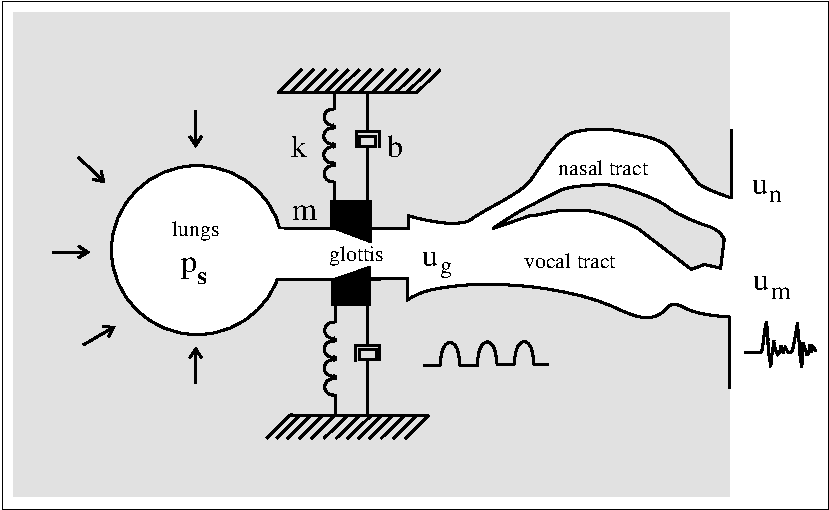
\includegraphics[width=80mm]{figure}}
\caption{{\it Speaker property distributions}}  
\label{dists}
\end{figure}

\subsection{Feature Selection}
\subsubsection{Audio}
We have tried three different types of features for audio, namely, openSMILE \cite{eyben}, MFCC and openSMILE + MFCC. The goal is to find the features that can characterize a speaker's variability. We used the same feature for each property estimation.

\begin{itemize}
\item openSMILE: there are 384 features including the characteristics for the signal energy, MFCC, zero-crossing rate, voice probability and F0. We found all five features useful, and we think these are instrumental to identify gender and age, etc.

\item MFCC: we used Kaldi's \cite{povey} \texttt{compute-mfcc-feats} utility to extract the MFCCs. These are 13 dimensional vectors extracted every 10ms. We randomly sampled 1000 vectors without replacement, then concatenate all of them to form a 13,000 dimensional feature vector.

\item openSMILE + MFCC: we concatenated the openSMILE and MFCC features together and form a 13,384 dimensional feature vector.
\end{itemize}

\subsubsection{Text}
KL distance is used for feature selection. If the exitence of a word $w$ can significantly increase the likelihood of being in class $c$, then $w$ is a discriminative feature. The KL distance of $w$ is computed as follows:
\begin{equation}
  KL(w) = D[p(c|w)||p(c)] = \sum_{c=1}^{C}p(c|w)\cdot log\frac{p(c|w)}{p(c)}.
\label{kl}
\end{equation}

We use the words with the highest KL distances as features. Given the smaller dataset we have, we only kept the words that are observed at least 3 times for each class.

In addition, we have three different approaches for scoring the features in each document $d$, which use tf-idf, augmented tf-idf and ``tf-kl hybrid'' scores respectively.
\begin{itemize}
\item tf-idf: this score is high when the word $w$ occurs many times in a small number of documents. Hence $w$ is highly discriminative in those documents.
\begin{equation}
  tf\textnormal{-} idf(t)^1 =tf_{t,d} \cdot idf_{t} 
\label{tfidf1}
\end{equation}

\item augmented tf-idf:  we calculate the augmented tf-idf score of a term $t$ as follows:
\begin{equation}
  tf\textnormal{-} idf(t)^2 = (0.5 + \frac{tf_{t,d}}{\underset{s}{\max}\, tf_{s,d}}) \cdot idf_{t} 
\label{tfidf}
\end{equation}

\item ``tf-kl hybrid'': we multiply the tf score of a term $t$ by its KL distance. Empirically, this method works better than tf-idf for this corpus.
\begin{equation}
  tf\textnormal{-} kl(t) = tf_{t,d} \cdot KL(t).
\label{tfkl}
\end{equation}
\end{itemize}


\subsection{Classifiers and Dimension Reduction}
We experimented with four different classifiers, which are k-NN, GMM, random forest and SVM. Two versions of classification packages are used, which are LIBLINEAR \cite{liblin} and LIBSVM \cite{libsvm}. For audio, we used the RBF kernel from LIBSVM. For text, we used the linear kernel from LIBLINEAR. The linear kernel is used for text because its feature vectors have relatively high dimensions, and nonlinear mapping doesn't improve the performance \cite{svmguide}. In addition, the linear kernel may run much faster. We also tried dimension reduction on the feature vectors using PCA whitening, and applied the new features to SVM.

\section{Experiments}
\subsection{Experimental Setup and Implementation Details}
We used 64\%/16\%/20\% split for train/validation/test sets. For each experiment, we train our model using the training set, and test the model on the validation set. We then select the model that generates the highest accuracy on the validation set, and produce the test accuracy on the test set. For both audio and text experiments, the datasets for train/validation/test are identical.

Again, for both audio and text, two sets of experiments are run for each. One is to fix the features and vary the classifier, the other is vice versa.

\subsection{Baselines}
For the classification problems for the four properties, we choose the percentage of the majority class in each property as its baseline estimation accuracy. For the regression problem on chronological age, we use the average age in the training set as the predicted age, then calculate MAE on test set using this age. The baselines are in Table \ref{baseline}.

\begin{table}
\caption{\label{baseline} {\it Baselines}}
\vspace{2mm}
\centerline{
\begin{tabular}{|c|c|}
\hline
Property & Accuracy \\ \hline \hline 
accent & 29.47\% \\
age (class.) & 33.52\% \\
gender & 55.62\% \\
education & 56.91\% \\
age (reg.) & 9.09 yrs \\
\hline
\end{tabular}}
\end{table}

\subsection{Audio}
\subsubsection{Classifiers}
We fix the features as openSMILE, and run four classifiers, with PCA whitening on the features for the SVM classifier. We varied different parameters for each classifiers. In particular, for SVM, the set of number of principle components we tried is \{50, 100, 150, 200, 250, 300, 350\}, the gammas is \{0.001, 0.01, 0.1, 1, 10\} and the regularization constant Cs is \{0.005, 0.05, 0.5, 5, 50\}. 
The test accuracies are shown in Table \ref{class_speech}.

\begin{table} [t,h]
\caption{\label{class_speech} {\it Test Accuracy for Different Classifiers in Speech (highest scores are in bold)}}
\vspace{2mm}
\centerline{
\begin{tabular}{|c|c|}
\hline
\multirow{2}{*}{Classifiers} & Test Accuracy (\%) \\
& accent/age/gender/edu \\ \hline \hline 
k-NN & 22.4 / 27.29 / 68.64 / 49.39 \\
GMM & 19.96 / 28.11 / \textbf{98.37} / 39.61 \\
random forest & 25.87 / 30.96 / 96.33 / 51.12 \\
SVC + PCA & \textbf{34.23} / \textbf{34.81} / 97.67 / \textbf{68.1} \\
\hline
\end{tabular}}
\end{table}

Table \ref{class_speech} shows SVC + PCA is superior on everything except for gender, where GMM is better. On age regression problem, we used SVR + PCA and achieved MAE of 8.22 years. We note all accuracies beat the baseline, and the best gender classification accuracy exceeds the baseline by 42.75\%.

\subsubsection{Features}
The above section shows SVM + PCA is mostly the best classifier, so we use it on different speech features. The results are shown in Table \ref{feats_speech}. We use the same range for gammas and Cs, but change the range for the number of principle components to \{50, 200, 500, 750, 1000, 3000, 5000, 7500, 10000, 12000\} for the last two features. 

\begin{table} [t,h]
\caption{\label{feats_speech} {\it Test Accuracy for Different Features in Speech (highest scores are in bold)}}
\vspace{2mm}
\centerline{
\begin{tabular}{|c|c|}
\hline
\multirow{2}{*}{Features} & Test Accuracy (\%) \\
& accent/age/gender/edu \\ \hline \hline 
openSMILE & \textbf{34.23} / \textbf{34.81} / \textbf{97.67} / \textbf{68.1} \\
MFCC & 31.46 / 29.96 / 90.28 / 56.41 \\
openSMILE + MFCC & 29.94 / 24.92 / 56.65 / 55.31 \\
\hline
\end{tabular}}
\end{table}

We discovered that openSMILE is the best audio feature among the three. The results show using the raw MFCC features won't increase the prediction accuracy. We need to obtain sophisticated derivatives of MFCCs such as the i-vectors to improve the performance.   

\subsection{Text}

\subsubsection{Classifiers}
We used KL divergence as the feature selection criterion, and ``tf-kl hybrid'' as the feature scoring function. We tried all 8 different classifiers provided by LIBLINEAR, and varied the regularization constant C in the set of \{0.01, 0.1, 1, 10\}. The results are shown in Table \ref{class_text}. We did not use GMM as we encountered the ``Out of memory'' problem. For SVC, we found that the best result is achieved without using PCA whitening. 

\begin{table} [t,h]
\caption{\label{class_text} {\it Test Accuracy for Different Classifiers in Text (highest scores are in bold)}}
\vspace{2mm}
\centerline{
\begin{tabular}{|c|c|}
\hline
\multirow{2}{*}{Classifiers} & Test Accuracy (\%) \\
& accent/age/gender/edu \\ \hline \hline 
k-NN & 25.49 / 31.43 / 71.13 / 61.82 \\
random forest  & 32.25 / \textbf{39.7} / 79.39 / 66.47 \\
SVC & \textbf{33.18} / 37.7 / \textbf{83} / \textbf{68.3} \\
\hline
\end{tabular}}
\end{table}

Table \ref{class_text} shows SVM is still mostly the best classifier among all three. On age regression problem, SVR achieves a MAE of 8.68 years. 

To compare with the best accuracy using the speech data shown in Table \ref{class_speech}, we can see the text features are marginally better on education level prediction; while the speech features are much better on gender, and slightly better on accent. For age, we could not decide which feature is better as the classification and regression results are different.

\subsubsection{Features}

\begin{table} [t,h]
\caption{\label{class_text} {\it Test Accuracy for Different Feature Scoring Methods (highest scores are in bold)}}
\vspace{2mm}
\centerline{
\begin{tabular}{|c|c|}
\hline
\multirow{2}{*}{Scoring Method} & Test Accuracy (\%) \\
& accent/age/gender/edu \\ \hline \hline 
tf-idf &   30.85/ 33.99/ 69.97/ 63.91 \\
augmented tf-idf  & 30.85 / 33.99 / 71.36 / 66.82 \\
tf-kl hybrid & \textbf{33.18} / \textbf{37.7} / \textbf{83} / \textbf{68.3} \\
\hline
\end{tabular}}
\end{table}

\subsubsection{Most Discriminative Words for Gender}
If we drop the summation in Equation \ref{kl} and sort its scores for a class $c$, we get the most discriminative words against $c$. Table \ref{genderdis} shows the top discriminative words for gender as an example.

\begin{table} [t,h]
\caption{\label{genderdis} {\it Most Discriminative Words for Gender}}
\vspace{2mm}
\centerline{
\begin{tabular}{|c|c|}
\hline
Male & Female \\ \hline \hline
wife's & husband's \\
metric & husband \\
constitution & sew \\
units & bake \\
mustang & dresses \\
baltimore & lovely \\
non & sewing \\
essentially & singing \\
economical & gorgeous \\
blade & babies \\
\hline
\end{tabular}}
\end{table}



\subsubsection{Speech Recognition System Simulation}
In recent speech recognition systems, the word error rate (WER) for the Switchboard corpus roughly ranges from 10\% to 25\% using deep neural network \cite{maas}. We are interested in using the transcribed speech generated from such a system to make prediction on the speakers properties. To simulate a real world speech recognition system, we swap each word in the dataset with a random word in the training set corpus with probability equal to the WER. The set of WERs (\%) we used is \{0, 10, 15, 20, 25\}.


\subsection{Combining Audio and Text Results}
For non-categorical variables, i.e., age and education level, we merge the predictions from audio and text by simply averaging them on the test set. Averaging makes sense in this case because the labels imply order for non-categorical variables. While this approach slightly improves the age classification accuracy, it doesn't improve or do worse on the education classification and age regression problems.

We also considered various methods such as Platt scaling \cite{platt} and isotonic regression to merge the results for categorical variables, namely, gender and accent. However, we did not implement the solution as it seems neither approach will produce a consistent answer with the SVM predictions. 

\section{Conclusions}


\eightpt
\bibliographystyle{IEEEtran}
\begin{thebibliography}{10}
\bibitem[1]{bahari} Bahari, M. H., et al., 
``Age Estimation from Telephone Speech using i-vectors'', 
Interspeech, 2012.

\bibitem[2]{dehak} Dehak, N., et al., 
``Front-End Factor Analysis for Speaker Verification'', 
IEEE Trans. Audio, Speech and Language Processing, 2011.

\bibitem[3]{garera} Garera, N. and Yarowsky, D.,
``Modeling Latent Biographic Attributes in Conversational Genres'',
ACL/IJCNLP, 2009

\bibitem[4]{boulis} Boulis, B and Ostendorf, M.,
``A Quantitative Analysis of Lexical Differences Between Genders in Telephone Conversations'',
ACL, 2005

\bibitem[5]{eyben} Eyben, F., Wöllmer, M. and Schuller, B.,
``openSMILE – The Munich Versatile and Fast Open-Source Audio Feature Extractor'',
ACM Multimedia, 2010

\bibitem[6]{povey} Povey, D., et al.,
``The Kaldi Speech Recognition Toolkit''.

\bibitem[7]{liblin} Fan, RE., et al.,
``LIBLINEAR: A Library for Large Linear Classification'',
JMLR, 2008

\bibitem[8]{libsvm} Chang, CC., et al.,
``LIBSVM: A Library for Support Vector Machines'',
ACM TIST, 2011

\bibitem[9]{maas} Maas, A.,  Hannun, A. and Yg, A.,
``Rectifier Nonlinearities Improve Neural Network Acoustic Models'',
ICML Workshop on Deep Learning for Audio, Speech, and Language Processing, 2013

\bibitem[10]{svmguide} Hsu, CW., Chang, CC. and Lin, CJ., 
``A Practical Guide to Support Vector Classification, Appendix C''.

\bibitem[11]{platt} Platt, J.,
``Probabilistic Outputs for Support Vector Machines and Comparisons to Regularized Likelihood Methods'',
Advances in Large Margin Classifiers, 1999

\end{thebibliography}
\end{document}
